\section{Theoretische Grundlagen}
\subsection{Biometrie und Biometrische Merkmale}
\subsectionauthor{Torben Brenner}
Bei der Biometrie handelt es sich um die Wissenschaft, die sich mit der Vermessung von biologischen Merkmalen beschäftigt \footcite[Vgl.][]{Sea18}. Dabei werden insbesondere in der Informationstechnologie Technologien zur Messung und Analyse von körperlichen Merkmalen untersucht.\newline
Diese Merkmale werden auch als biometrische Merkmale bezeichnet. Dabei wird unterschieden zwischen den verhaltensbasierten und den physiologischen Merkmalen(Vgl. \cite{Sas06}). Erstere zeichnen sich dadurch aus, dass eine Person aktiv eine Handlung ausführen muss um das Merkmal zu zeigen, während dem die physiologischen Merkmale dauerhaft von einer Person getragen werden. Ein Beispiel für verhaltensbasierte Merkmale ist die Gangart eines Menschen, die sogar zur Authentifizierung verwendet werden kann (Vgl. \cite{Cla09}). Ein bekanntes physiologisches Merkmal ist der Fingerabdruck einer Person.\newline
Ein häufiger Einsatzzweck der Biometrie ist die Authentifizierung eines Nutzers gegenüber einem System. Da sich nicht alle Merkmale für eine solche Identifikation eignen, müssen verschiedene Faktoren bei der Auswahl der Merkmale betrachtet werden. \cite{Akj04} nennt zum Beispiel folgende Faktoren: 
\begin{itemize}
	\item \textbf{Universalität}: Jeder Mensch sollte dieses Merkmal besitzen.
	\item \textbf{Unterscheidbarkeit}: Das Merkmal soll sich so stark wie möglich zwischen zwei Personen unterscheiden.
	\item \textbf{Permanenz}: Das Merkmal sollte sich über die Zeit betrachtet nicht oder nur in geringem Maße ändern.
	\item \textbf{Erfassbarkeit}: Das Merkmal sollte möglichst einfach dauerhaft erfasst werden können.
	\item \textbf{Performanz}: Beschäftigt sich mit der Frage mit welchem Zeitaufwand und mit welcher Geschwindigkeit ein Merkmal gemessen werden kann. 
	\item \textbf{Akzeptanz}: Beschäftigt sich mit der Frage in wie weit Nutzer mit der Messung eines Merkmals einverstanden sind. 
	\item \textbf{Umgehbarkeit}: Beschäftigt sich mit der Frage, in wie weit ein Nutzer dem System vortäuschen kann das er ein anderer Nutzer ist.
\end{itemize}
Die ersten vier Faktoren beschäftigen sich im Allgemeinen mit der Eignung eines Merkmals für die Authentifizierung, während sich die letzten Faktoren mit der Eignung eines Biometrischen Systems für eine Aufgabe beschäftigen. Da sich unsere Fragestellung aber nicht auf die Authentifizierung eines Nutzers gegenüber eines Informationstechnischen Systems bezieht, sondern sich mit der Auswertung der erfassten Daten für die Erkennung von Emotionen beschäftigt, ist der Faktor der \textit{Unterscheidbarkeit} zu vernachlässigen. Die restlichen Faktoren werden aber später für die einzelnen biometrischen Merkmale untersucht wobei sich die Faktoren \textit{Performanz, Akzeptanz und Umgehbarkeit} auf die Messung mit Smartphones beziehen.
\subsection{Emotionen}
\subsubsection{Definition}
\subsubsectionauthor{Torben Brenner}
Da wir uns in dieser Arbeit mit der Erkennung von Emotionen beschäftigen, ist es notwendig, dass wir den Begriff der Emotion definieren. Das Problem an dem Begriff der Emotion ist, dass diese ein Hypothetisches Konstrukt ist, welches sich aus der physiologischen Erregung, dem motorischen Ausdruck, Handlungstendenzen und einem subjektiven Gefühl zusammensetzt (\cite{Kla02}[Vgl.][S.166 Abschnitt Emotion]).\newline
Als Beispiel nennt Klaus Scherer hier das plötzliche Auftreten eines Mannes mit einem Blut verschmierten Messer beim Sonntagsspaziergang. Er beschreibt daraufhin welche Aspekte in diesem Szenario eine Rolle spielen. So kann zum einen eine physiologische Reaktion gemessen werden, in Form eines erhöhten Herzschlages. Außerdem wird eine motorische Reaktion stattfinden, z.Bsp. weit aufgerissener Mund und Augen. Die Handlungstendenz wäre in seinem Beispiel der plötzliche Drang wegzulaufen und bei der späteren Befragung zu dieser Situation könnte eine Person sagen, dass sie Furcht gefühlt hat.
\subsubsection{Grundlagen der Emotionserkennung}
\subsectionauthor{Torben Brenner}
Nach dem nun geklärt ist was unter einer Emotion verstanden wird, stellt sich die Frage wie man diese erkennen kann. Das Problem hierbei ist, dass es eine große Anzahl an Emotionen gibt, laut Hokuma\footcite[Vgl.][Absch. 1]{Hok17} sind es 34.000 unterschiedliche Emotionen. Diese verschiedenen Emotionen lassen sich nur schwer erfassen und unterscheiden, weshalb ein Weg gefunden werden muss die Emotionen einzuteilen. Diese Einteilung wurde bereits von Robert Plutchick vorgenommen und herausgekommen sind dabei acht primäre Emotionen: Freude, Traurigkeit, Akzeptanz, Ekel, Angst, Wut, Überraschung und Erwartung.\newline
Mit diesen acht Emotionen hat Plutchick das Rad der Emotionen gebildet(siehe Abbildung).
\begin{figure}[h]
	\centering
	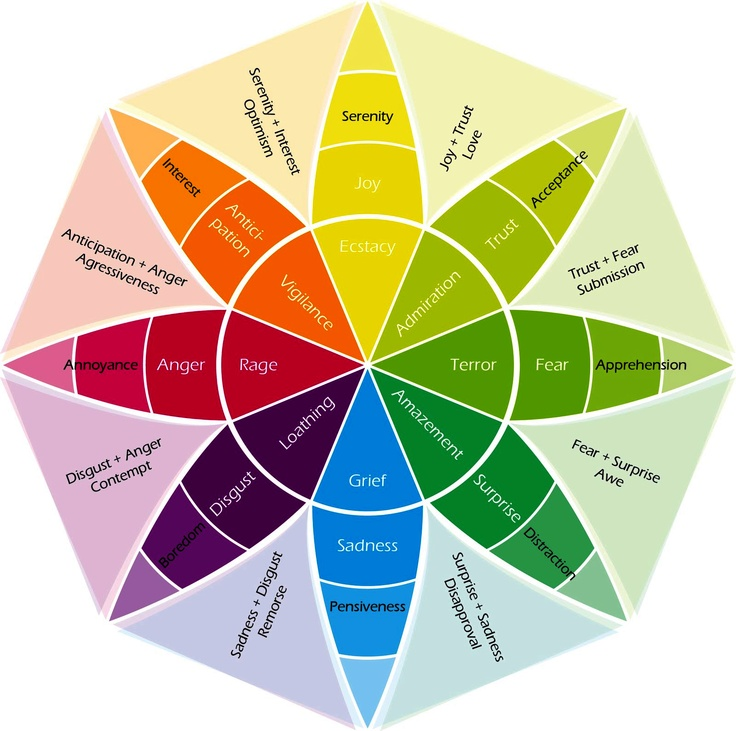
\includegraphics[width=16cm]{Bilder/wheel-of-emotions.png}
	\caption[Rad der Emotionen - Robert Plutchick]{Rad der Emotionen - Robert Plutchick\footnotemark}
\end{figure}%
\footcitetext[Vgl.][]{Hok17}
\newline
Das Rad stellt die primären Emotionen dabei in Relation, wobei die Kombinationen zwischen zwei Emotionen im Raum zwischen diesen steht und Emotionen die gegensätzlich wirken, z. Bsp. Traurigkeit und Freude, jeweils auch gegenüberliegend auf dem Rad sind. Außerdem wird die Stärke einer Emotion durch deren nähe zum Zentrum des Rads gekennzeichnet, z. Bsp. Wut zu toben \footcite[Vgl.][Absch. Elements of the Wheel]{Hok17}.\newline
In der Literatur gibt es neben dem Model von Plutchick auch das \textit{Gevena Emotion Wheel}. Dieses Modell betrachtet die Emotionen nicht in acht primären Hauptkategorien, sondern unterscheidet zwischen 20 Emotionen anhand von zwei Parametern, die Valenz und die Kontrolle. Die Kontrolle bezeichnet, wie stark Individuum eine Situation kontrollieren kann. Die Valenz sagt aus ob eine Situation für das Individuum eher angenehm oder unangenehm ist.\newline 
Beide Modelle können dafür genutzt werden um Emotionen auszuwerten, wobei hier zu diskutieren ist welches Modell besser geeignet ist.
\subsection{Umgang mit biometrischen Daten}
\subsectionauthor{Torben Brenner}
Eine Problematik, mit der wir uns in dieser Arbeit beschäftigen müssen, ist der Umstand das biometrische Daten nicht immer einen direkten Schluss auf einen Emotion zulassen. So lässt ein hochfrequenter Puls keinen direkten Schluss auf die Emotion zu, die ein Individuum gerade empfindet. Er kann maximal ein Indiz für verschiedene Emotionen sein, z. Bsp. Wut oder Angst. Um mit diesem Umstand umzugehen benötigen wir zwei neue Begriffe die im folgenden genauer erläutert werden. 
\subsubsection{Indiz}
Ein Indiz ist im allgemeinen Sprachgebrauch ein Anzeichen für einen Umstand, an dem sich ein Zustand oder eine Entwicklung absehen lässt\footcite[Vgl.][]{Dud18}. In unserer Arbeit, sehen wir Daten die wir von den Sensoren bekommen, als Indizien an. Ein Indiz macht es wahrscheinlicher bzw. unwahrscheinlicher das ein Individuum eine bestimmte Emotion verspürt. 
\subsubsection{Kausalität}
Als Kausalität wird im allgemeinen der Zusammenhang zwischen Ursache und Wirkung verstanden. In der Physik ist die Kausalität ein grundlegendes Prinzip, welches besagt, ``daß in der Natur nichts ohne Grund passiert, d.h. zu jedem Ereignis (Wirkung) ein anderes (Ursache) existiert, das a) in seiner Vergangenheit liegt und b) zwingende Voraussetzung für das Eintreten der Wirkung ist''\footcite{Sav18}.\newline
In dieser Arbeit werden wir ebenfalls versuchen, kausale Zusammenhänge zwischen Reaktionen des Körpers und den gerade empfundenen Emotionen zu ermitteln.
Ein Werkzeug um kausale Zusammenhänge darzustellen ist in der Literatur der Kausale Graph (im englischen \textit{directed acyclic graph}).
\begin{figure}[h]
	\centering
	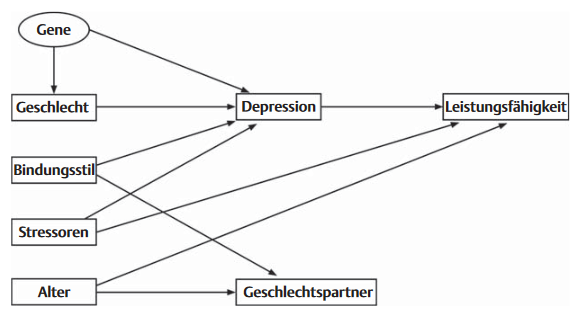
\includegraphics[width=11cm]{Bilder/dag.png}
	\caption[Fiktives Beispiel eines DAGs]{Fiktives Beispiel eines DAGs\footnotemark}
\end{figure}
\footcite[Vgl.][Kausale Graphen - DAGs]{Tho11}
Die Grafik zeigt ein fiktives Beispiel für einen kausalen Graphen. In diesem Beispiel von Thoemmes wird dargestellt das Bindungsstil, Geschlecht, Stressoren und Gene Einfluss auf Depressionen haben. Wichtig ist, dass alle Annahmen die in einem solchen Graph gemacht werden theoretisch begründet werden müssen. Ist dies nicht der Fall, dürfen sie kritisiert und infrage gestellt werden \footcite[Vgl. ][S.3 Kausale Graphen - DAGs]{Tho11}.
\subsection{Emotionsindizien}
\subsubsection{Puls}
In diesem Abschnitt beschäftigen wir uns mit dem Puls als ein Indiz für verschiedene Emotionen. Hierbei wird der als der biologische Puls gesehen, das heißt ``die in Abhängigkeit vom Herzrhythmus (Herzmechanik) erfolgende Schwankung von Blutstrom, Blutdruck oder Blutvolumen im Blutkreislaufsystem (Blutgefäßsystem, Blutkreislauf)''\footcite{Spe18}. Neben dieser Defioniton wird im Lexikon der Biologie auch folgende Definition genannt: ``die vom Herzschlag bewirkte, rhythmisch auftretende Druckwelle (Pulsschlag) in den Arterien''\footcite{Spe18}, welche den Puls als ateriellen Puls definiert. \newline
Die Messung des Pulses wird auch als Sphygmologie bezeichnet.
\subsubsection{Hautleitfähigkeit/Hautwiderstand}
\subsubsectionauthor{Lukas Seemann}
Die menschliche Haut verfügt über \glqq \textit{aktive als auch passive elektrische Eigenschaften, die sich auf Strukturen und Fuktionen der Haut und der in ihr enthaltenen Organe zurückführen lässt.}\grqq{}\footcite[][S. 2]{Bou88} Diese elektrischen Phänomene der Haut sind in wissenschaftlichen Kreisen unter dem Sammelbegriff elektrodermale Aktivität (kurz EDA) bekannt. \footcite[Vgl.][S. 2]{Bou88}
Eine elektrodermale Aktivität, die sich sehr gut als Indikator für Emotionen eignet, ist die Hautleitfähigkeit. Hierzu wird mit einer externen Stromquelle mit geringer Spannung gemessen, wie gut die Haut eines Probanden diesen Strom leitet. \footcite[Vgl. ][S.77]{Moe07} Häufig wird anstand der Hautleitfähigkeit auch der Hautwiderstand gemessen. Diese beiden Indizien stehen in einer negativ proportionalen Beziehung. Dies bedeutet, je höher der Widerstand der Haut ist, desto niedriger ist die Leitfähigkeit und umgekehrt. Letzten Endes sagen beide Indizien dasselbe aus, unterscheiden sich aber in der Betrachtungsrichtung. \footcite[Vgl. ][S. 28]{Die06} \newline
Die Hautleitfähigkeit wird anhand der Menge von Schweiß an den Ausgängen der Schweißdrüßen bestimmt, die sich über den gesamten Körper veteilen. Je mehr Schweiß, der elektrisch sehr gut leitend ist, sich auf der Haut befindet, umso größer ist die Hautleitfähigkeit. Am besten eignen sich  Stellen, an denen die Schweißdrüsen sehr dicht angeordnet sind und die somit sehr schweißsensibel sind. Dies ist zum Beispiel an den Handinnenflächen beziehungsweise Fingerinnenseiten der Fall, die sich deshalb sehr gut für solche Messungen eignen. \footcite[Vgl. ][S.77]{Moe07} 
\begin{figure}[h]
	\centering
	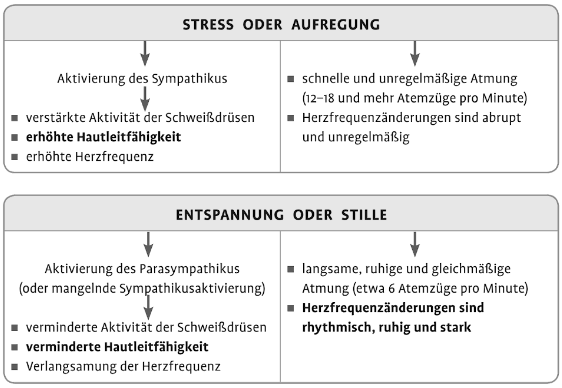
\includegraphics[width=14.6cm]{Bilder/symp.png}
	\caption[Reaktion des Körpers auf Stress und Entspannung]{Reaktion des Körpers auf Stress und Entspannung\footnotemark}
\end{figure}%
\footcitetext[][S. 200]{Dil13}
\newline
\glqq \textit{Die Aktivation beschreibt das Ausmaß der physiologischen Aktiviertheit oder Wachheit eines Menschen}\grqq{}\footcite[][S. 28]{Die06}. Unter Aktivitation versteht man bei Menschen generell jede Art von emotionaler Erregung. Hierzu zählen unter anderem Wut, Aufregung, Schreckmomente oder auch extreme Freude. In Abbildung 3 ist die Reaktion des Körpers auf Stress (darausfolgend auch Aktivation) und auf Entspannung dargestellt. Die Schweißprodukation wird über das unwillkürliche Nervensystem gesteuert. Dieses besteht aus Sympathikus der für die Bereitstellung von Energie und Arbeitsleistungs zustöndig ist, und dem Parasympathikus, der zur Erholung und Wiederherstellung von Körperfunktionen dient. \footcite[Vgl. ][S. 5]{Lie13} \newline Bei Stress oder Aufregung wird der Sympathikus aktiviert, was eine versträkt Schweißproduktion und somit auch eine erhöhte Hautleitfähigkeit hervorruft. Außerdem wird die Herz- und Atemfrequenz erhöht und der Rhymtmus dieser ist unregelmäßig. Die Reaktion auf ein Ereignis, das emotionale Erregung hervorruft, lässt sich meistens innerhalb von einer bis vier Sekunden anhand der Änderung der Hautleitfähigkeit feststellen. \footcite[Vgl.][S. 130f]{Sch14} \newline 
Bei Entspannung hingegen wird der Parasympathikus aktiviert, was zu einer verminderten Aktivität der Schweißdrüßen führt. Die Hautleitfähigkeit sinkt somit auch. Des Weiteren werden Herz- und Atem verlangsamt und gelangen wieder in einen normalen Rhymthmus. \newline
Der Vorteil der Messung der Hautleitfähigkeit ist, dass diese unwillkürlich gesteutert wird und somit keine willentliche Mitarbeit des Probanden erfodert. Da die Aktivierung des Sympathikus automatisch geschieht, kann der Proband die Messung nicht verfälschen. \newline
Ein Nachteil des Verfahren ist, dass die Hautleitfähigkeit nur Rückschlüsse auf den Grad der Aktiviation schließen lässt, jedoch nicht gesagt werden kann, ob es sich um positive oder negative Reaktionen handelt. Die Wut über ein Ereignis würde zum selben Ergebnis führen, wie die übermäßige Freude über ein Ereignis. Aus diesem Grund müssen zur genauen Emotionsbestimmung weitere Indizien herangezogen werden. \footcite[Vgl. ][S.77]{Moe07}
\subsubsection{Gesichtszüge}
\subsubsection{Tippverhalten}
\subsubsectionauthor{Torben Brenner}
Besitzer eines Smartphones verwenden dieses für die verschiedensten Lebensaufgaben. Neben der Hauptaufgabe, dem telefonieren, wird das Smartphone sowohl zum Nachrichten schreiben als auch für das Bilder machen verwendet. Dabei lassen sich theoretisch Daten wie die Tippgeschwindigkeit erfassen, oder aber auch mit Einwilligung des Nutzers der Text versendeter Nachrichten analysieren.
\subsection{Hardware zur Erfassung von biometrischen Daten}
\subsubsection{Smartphones}
\subsubsectionauthor{Torben Brenner}
Ein Smartphone differenziert sich durch mehrere Aspekte von einem herkömmlichen Telefon. Der erste Unterschied, so wie alten mobil Telefonen, ist das Telefonieren ohne direkten Kabelanschluss an das Netz oder zusätzliche Basisstation.\newline 
Wodurch es sich aber von den eben genannten mobil Telefonen unterscheidet, ist die Leistungsfähigkeit der einzelnen Komponenten. So besitzen heutige Smartphones häufig Prozessoren mit Acht Kernen und Leistungen ab 1,7 GHz pro Kern. Neben der Leistungsfähigkeit des Prozessors ist auch die Menge des verbauten Hauptspeichers gewachsen. Die wenigsten Smartphones besitzen heute noch weniger als 2 Gigabyte Arbeitsspeicher. Diese stärkeren Komponenten ermöglichen das ausführen komplexer Anwendungen und außerdem Multitasking. Das lässt beim Vergleich mit der Definiton eines Computers es auch zu, zu behaupten das Smartphones ebenfalls Computer sind. \textbf{TODO: das hier mit quellen und bezug auf die beiden definitionen}\newline
Der Hauptunterschied ist aber die Menge der verbauten Sensoren. Wie Kai Biermann auf Zeit Online schreibt, ermöglichen diese es einem Smartphone zu sehen, fühlen und hören \footcite[Vgl.][S. 1 Abs. 2]{Bie14}. In diesem Artikel beschreibt Biermann die enormen Möglichkeiten die diese Sensoren ermöglichen. So ermöglicht ein Smartphone die Navigation per Positionsbestimmung, das Mikrofon das hören und die Handykamera ermöglicht dem Smartphone das sehen. Gerade weil Smartphone Kameras immer besser werden sind die Möglichkeiten zur Gesichtserkennung deutlich gestiegen, wie zuletzt Apple mit dem IPhone X zeigte, das Emotionen über die Kamera erkennt und diese auf die sogenannten Animojis überträgt. \textbf{TODO: Finde Quelle für diese Aussage} \newline
% Ursprünglich aus anderem Kapitel
Wie bereits erwähnt, sind in Smartphones sehr viele unterschiedliche Sensoren verbaut. Diese ermöglichen es dem Smartphone den Zustand seiner Umwelt zu erfassen und somit auch Informationen über den Nutzer in Form von Daten zu erhalten. \newline
So gibt es aktuell so gut wie keine Smartphones mehr, die ohne einen Kamera oder Gyrosensor auf den Markt kommen. Die Kamera, kann z. Bsp. zum analysieren der Gesichtsgeometrie einer Person verwendet werden. Der Gyrosensor bietet verschiedene Möglichkeiten Informationen über eine Person zu erfassen, so könnte er zum einen zur Erfassung des Gangstils (engl. \textit{automatic gait recognition}) verwendet werden oder unterstützend bei der Analyse des Tippverhaltens wirken. So könnte analysiert werden, mit welcher Stärke ein Nutzer seine Nachrichten eingibt was unter anderem ein Indiz für Aggression, also Wut wäre. 
\subsubsection{Sensoren}
\subsubsectionauthor{Torben Brenner \& Lukas Seemann}
Sensoren dienen zur Erfassung eines physikalischen Zustandes und der Transformation dieses Zustandes in einen Impuls der verarbeitet werden kann\footcite[Vgl.][]{Web18}. In der Computertechnik, dienen Sensoren häufig dazu, den physikalischen Zustand verständlich für einen Computer zu machen, in dem dieser in einen Datensatz umgewandelt wird. \newline 
%Ursprünglich aus anderem Kapitel hizugefügt
Die bereits in Kapitel 2.4.2 beschriebene elektrodermale Aktivität kann mithilfe von EDA-Sensoren gemessen werden. Diese Art von Sensoren sind üblicherweise nicht in Smartphones eingebaut, weswegen die Hautleitfähigkeit mit externer Hardware gemessen werden muss. \newline
Die für heute eher unübliche Messungsart der elektrodermalen Aktivität stellt die endosomatische Messung dar. Indem winizige Elektroden in die Haut eingestochen werden, kann die Aktivität der Nerven in der Haut gemessen werden. \footcite[Vgl.][Folie 25]{Sch12} Hierbei handelt es sich jedoch nicht um eine Messung der Hauteleitfähigkeit sondern um eine Messung des Hautpotenzials. \newline
Bei der exosomatischen Messung hingegen wird ein schwacher Strom von ungefähr 0.5 Volt an die Haut angelegt. Die Spannung wird hierbei konstant gehalten, wodurch die Leitfähigkeit der Haut gemessen werden kann. Hierbei gemessen wird entweder in der Einheit Siemens für den elektrischen Leitwert oder in Ohm für den Widerstand. Die Elektroden des Sensor sind meistens aus Silber oder Silberchlorid und werden meist an zwei Stellen der nicht dominanten Hand angebracht. \footcite[Vgl.][Folie 25]{Sch12} Wie in Abbildung ? dargestellt gibt es verschiedenen Möglichkeiten der Handinnenfläche, die gut geeignet sind, (\#1, \#2 oder \#3). \newline 
\begin{figure}[h]
	\centering
	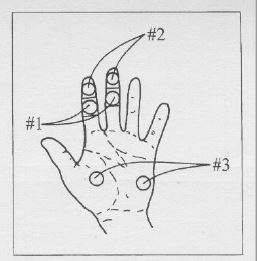
\includegraphics[width=12cm]{Bilder/gsr-hand.jpg}
	\caption[Positionsmöglichkeiten der EDA-Messung]{Positionsmöglichkeiten der EDA-Messung\footnotemark}
\end{figure}\footcitetext[][Folie 25]{Sch12}
\newline
Diese Art von Sensoren sind die heutzutage übliche Vorgehensweise bei EDA-Messungen. Häufig sind sie auch unter dem Namen GSR-Sensor\footnote{GSR: Galvanic Skin Response} bekannt und darunter im Internet erhältlich. GSR-Sensoren sind als Modul für den Mikrocontroller Arduino verfügbar.\footcite[beispielsweise:][]{Gro18} Dies stellt eine Möglichkeit dar, einem mobilen Endgerät die Sensordaten zum Beispiel über Bluetooth oder WiFi zur Verfügung zu stellen. In Abbildung ? ist ein GSR-Sensor inklusive der Elektroden für die Fingerinnenseiten, der mit Arduinos kompatibel ist, abgebildet.
\begin{figure}[h]
	\centering
	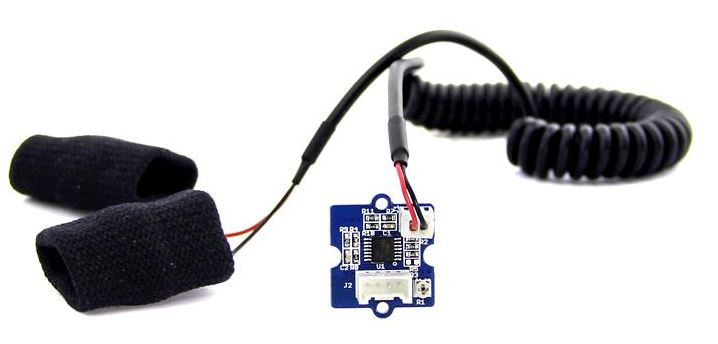
\includegraphics[width=15cm]{Bilder/sensor.jpg}
	\caption[GSR-Sensor mit Finger-Elektroden]{GSR-Sensor mit Finger-Elektroden\footnotemark}
\end{figure}%
\footcitetext{Gro18}
